\usetikzlibrary{calc}
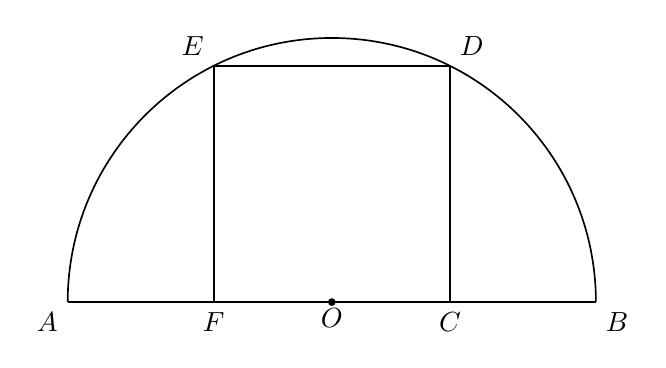
\begin{tikzpicture}[x=1cm,y=1cm,line width=.6pt,font=\normalsize]
\coordinate (O) at (0,0);
\coordinate (A) at (-3.3541019662496847,0);
\coordinate (B) at (3.3541019662496847,0);
\coordinate (F) at (-1.5,0);
\coordinate (C) at (1.5,0);
\coordinate (E) at (-1.5,3);
\coordinate (D) at (1.5,3);
\draw (A) arc[start angle=180,end angle=0,radius=3.3541019662496847cm];
\draw (A)--(B);
\draw (F)--(E);
\draw (C)--(D);
\draw (E)--(D);
\node[below left] at (A) {$A$};
\node[below right] at (B) {$B$};
\node[below] at (F) {$F$};
\node[below=2pt,inner sep=0pt] at (O) {$O$};
\node[below] at (C) {$C$};
\node[above left] at (E) {$E$};
\node[above right] at (D) {$D$};
\fill (O) circle[radius=1.4pt];
\end{tikzpicture}
